\documentclass{article}

\usepackage[utf8]{inputenc}
\usepackage[T1]{fontenc}
\usepackage{lmodern}
\usepackage{amsmath}
\usepackage{amsfonts}
\usepackage{amssymb}
\usepackage{booktabs}
\usepackage{graphicx}
\usepackage{hyperref}

\title{Exact-Polar Muon vs. Finite-Step Newton--Schulz Muon}
\author{}
\date{}

\begin{document}
\maketitle

\begin{abstract}
This note compares two versions of Muon's orthogonalization step. The usual
implementation in this repository uses a finite number of quintic
Newton--Schulz steps, which approximates the polar factor. The exact-polar
ablation computes an SVD and sets every live singular value to one exactly.
The experiment asks whether Muon's behavior comes from the exact polar ideal
\(UV^\top\), or from the softer finite-step Newton--Schulz approximation.
\end{abstract}

\section{The Two Orthogonalizers}

Let \(M \in \mathbb{R}^{m\times n}\) be the momentum or Nesterov momentum
matrix. Write its compact singular value decomposition as
\[
    M = U \Sigma V^\top,
    \qquad
    \Sigma = \operatorname{diag}(\sigma_1,\ldots,\sigma_k),
    \qquad
    k=\min(m,n).
\]

\paragraph{Exact-polar Muon.}
The exact polar update is
\[
    D_{\mathrm{svd}} = U V^\top.
\]
For every live singular direction, this sets
\[
    \sigma_i(D_{\mathrm{svd}})=1.
\]
This is the literal ``put all singular values to one'' version.

\paragraph{Newton--Schulz Muon.}
The practical Muon baseline avoids the SVD. It first normalizes
\[
    X_0 = \frac{M}{\|M\|_F+\varepsilon}
\]
and then applies the quintic Newton--Schulz-style iteration
\[
    X_{j+1}
    =
    2X_j
    -
    1.5(X_jX_j^\top)X_j
    +
    0.5(X_jX_j^\top)^2X_j.
\]
On singular values, this is the scalar map
\[
    q(\sigma)
    =
    2\sigma - 1.5\sigma^3 + 0.5\sigma^5.
\]
The repository's standard Muon config uses \(12\) such steps.

\section{Scalar Response}

The exact-polar path maps every nonzero singular value directly to \(1\). In
contrast, finite-step Newton--Schulz only approaches this behavior. For very
small singular values, the scalar map is approximately linear:
\[
    q(\sigma) \approx 2\sigma
    \qquad
    \text{when } \sigma \ll 1.
\]
After \(12\) steps, tiny singular values are therefore amplified by about
\[
    2^{12}=4096,
\]
not sent all the way to \(1\).

\begin{figure}[t]
    \centering
    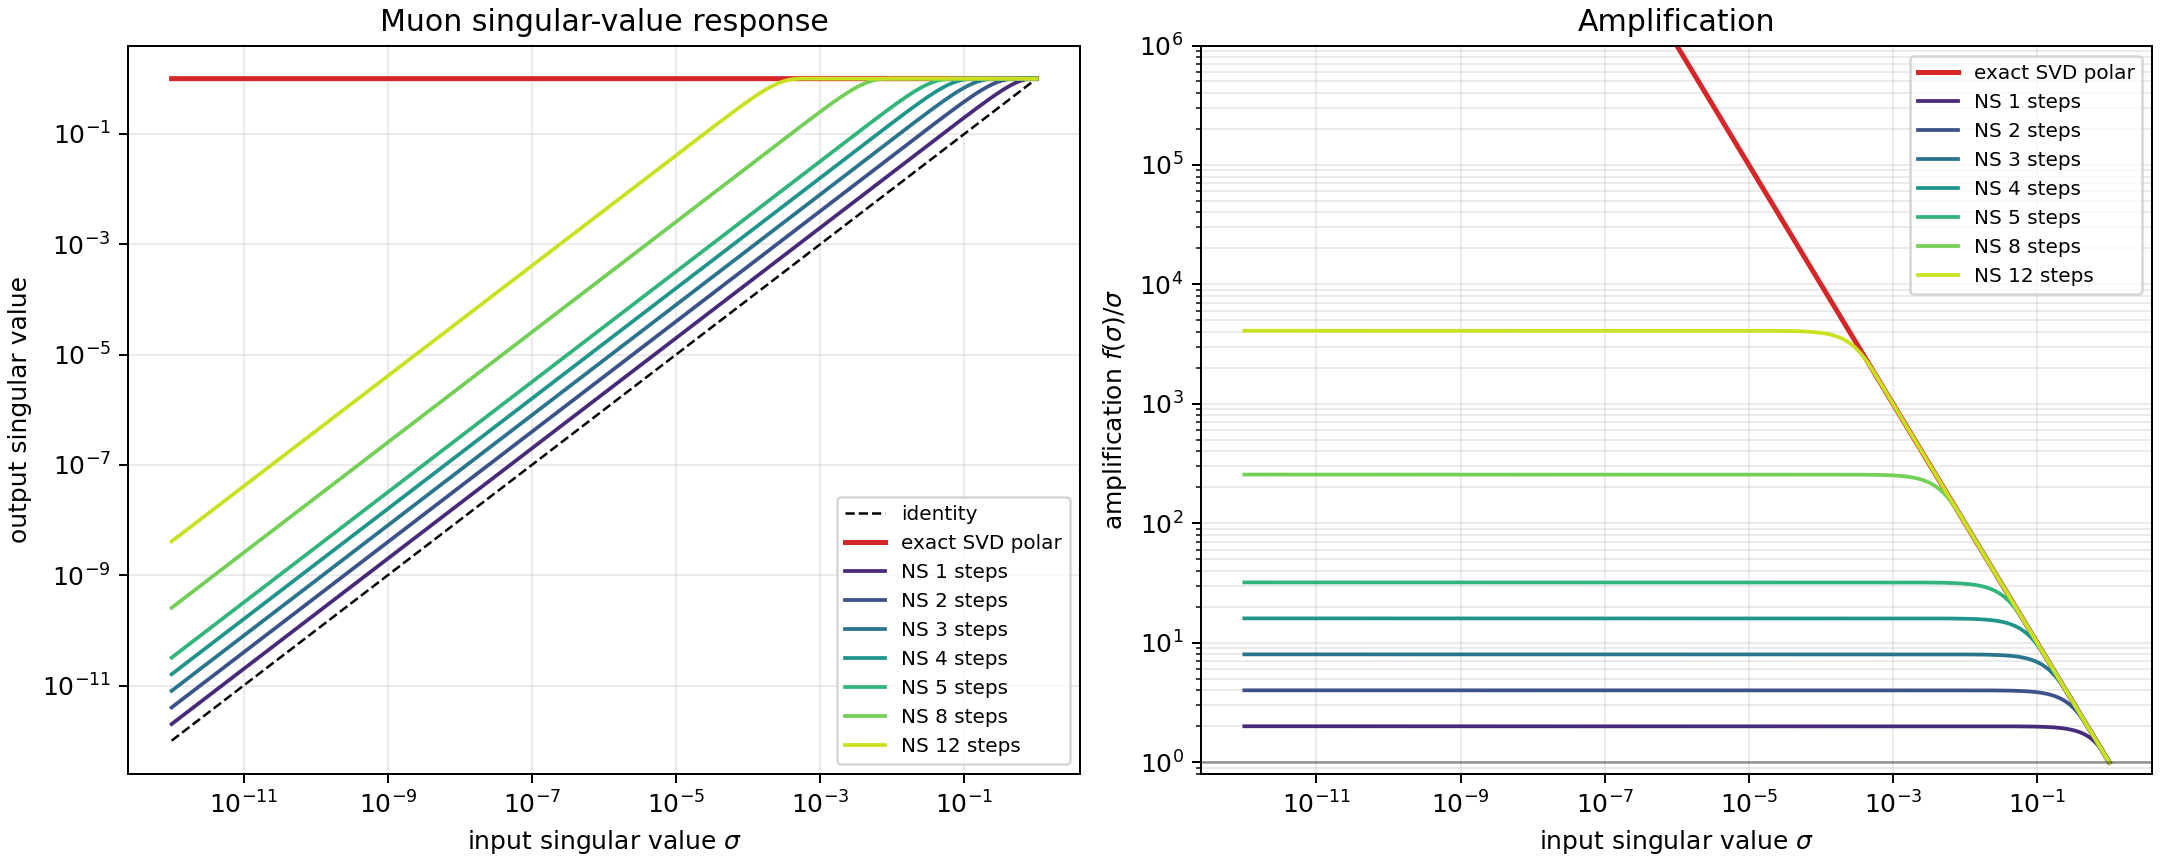
\includegraphics[width=\linewidth]{results/muon_svd_vs_ns_steps.png}
    \caption{Singular-value response of exact-polar Muon versus finite-step
    quintic Newton--Schulz Muon. The exact SVD polar update sends every live
    singular value to \(1\). The NS approximation reaches \(1\) quickly for
    moderate singular values, but leaves very small directions below \(1\)
    after a finite number of steps.}
    \label{fig:muon-svd-vs-ns}
\end{figure}

\begin{table}[t]
\centering
\begin{tabular}{rrrr}
\toprule
input \(\sigma\) & NS, 5 steps & NS, 12 steps & exact SVD polar\\
\midrule
\(10^{-8}\) & \(3.2\cdot 10^{-7}\) & \(4.1\cdot 10^{-5}\) & \(1\)\\
\(10^{-7}\) & \(3.2\cdot 10^{-6}\) & \(4.1\cdot 10^{-4}\) & \(1\)\\
\(10^{-6}\) & \(3.2\cdot 10^{-5}\) & \(4.1\cdot 10^{-3}\) & \(1\)\\
\(10^{-5}\) & \(3.2\cdot 10^{-4}\) & \(4.1\cdot 10^{-2}\) & \(1\)\\
\(10^{-4}\) & \(3.2\cdot 10^{-3}\) & \(3.9\cdot 10^{-1}\) & \(1\)\\
\(10^{-3}\) & \(3.2\cdot 10^{-2}\) & \(1.0\) & \(1\)\\
\bottomrule
\end{tabular}
\caption{Representative singular-value outputs for the repository's Muon
Newton--Schulz polynomial versus exact SVD polar orthogonalization.}
\end{table}

\section{Experiment}

The code now exposes this as a Muon option:
\[
    \texttt{orthogonalize} \in \{\texttt{ns},\texttt{svd}\}.
\]
The baseline uses
\[
    \texttt{orthogonalize: ns},
    \qquad
    \texttt{ns\_steps: 12}.
\]
The exact-polar ablation uses
\[
    \texttt{orthogonalize: svd}.
\]
Both variants keep the same momentum, Nesterov update, shape-aware learning
rate scaling, weight decay, and AdamW fallback groups. Thus the intended
comparison is finite-step NS soft polar versus exact SVD polar, where the
exact SVD path sets all live singular values to one.

\end{document}
